%% Template for SDP report, adapted from mlp_cw2_template, 2018. 

%% Based on  LaTeX template for ICML 2017 - example_paper.tex at 
%%  https://2017.icml.cc/Conferences/2017/StyleAuthorInstructions

\documentclass{article}
\usepackage[T1]{fontenc}
\usepackage{amssymb,amsmath}
\usepackage{txfonts}
\usepackage{microtype}
\usepackage{xspace}
\xspaceaddexceptions{\%}

% Lists with less spacing between items
\usepackage{paralist}

% For figures
\usepackage{graphicx}
\usepackage{subfig} 

% For citations
\usepackage{natbib}

% For algorithms
\usepackage{algorithm}
\usepackage{algorithmic}

% the hyperref package is used to produce hyperlinks in the
% resulting PDF.  If this breaks your system, please commend out the
% following usepackage line and replace \usepackage{mlp2017} with
% \usepackage[nohyperref]{mlp2017} below.
\usepackage{hyperref}
\usepackage{url}
\urlstyle{same}

% Packages hyperref and algorithmic misbehave sometimes.  We can fix
% this with the following command.
\newcommand{\theHalgorithm}{\arabic{algorithm}}


% Set up MLP coursework style (based on ICML style)
\usepackage{mlp2018}
\mlptitlerunning{SDP Demo \demoNumber  Group (\groupNumber)}
\bibliographystyle{icml2017}


\DeclareMathOperator{\softmax}{softmax}
\DeclareMathOperator{\sigmoid}{sigmoid}
\DeclareMathOperator{\sgn}{sgn}
\DeclareMathOperator{\relu}{relu}
\DeclareMathOperator{\lrelu}{lrelu}
\DeclareMathOperator{\elu}{elu}
\DeclareMathOperator{\selu}{selu}
\DeclareMathOperator{\maxout}{maxout}







%% You probably do not need to change anything above this comment

%% REPLACE the details in the following commands with your details
\setGroupNumber{18}
\setGroupName{Opticane}
\setProductName{Opticane}
\setDemoNumber{2}
\setLogoFileName{figs/opticane-logo.png}

\begin{document}

\makeSDPTitle{Demo}

% Previous MLP Style Title Layout working. 
% \twocolumn[
    % \mlptitle{\productName: SDP Demo \demoNumber}
    % \centerline{Group \groupNumber: \groupName}
% ]

\begin{abstract}
Opticane is a cane for the visually impaired that translates a user's surroundings to haptic feedback in the handle.

For the second demo, we've made significant progress in software, hardware, 3D modeling, simulation, and background research. We've parsed LIDAR output, established communication between LIDAR output and an LED array in-person, created a 3D model of Opticane's handle, modeled multiple simulations with humans to demonstrate real-world scenarios, conducted literature review, and reached out to organizations who interact with the visually impaired.
\end{abstract}

\section{Project Plan Update} 

From our last demo, the goals that we planned to achieve for this demo were:
\begin{itemize}
    \item Hardware 2.1: LIDAR to LED communication in-person (achieved)
    \item Hardware 2.2: Deciding of hardware components for ordering (achieved)
    \item Software 2.1: Interpret LIDAR data in-person (achieved)
    \item Simulation 2.1: LIDAR to LED communication in simulation (partially achieved)
    \item Design 2.1: Create initial designs for tactile feedback (achieved)
\end{itemize}

Our group was able to achieve all of these goals except for shifting goal "Simulation 2.1" because we chose to use console output to model the LIDAR output instead of simulated LEDs. This achieves the same semantic purpose of visually demonstrating our ability to interpret and simplify LIDAR data. LIDAR to LED communication in person, however, was still achieved.

While working towards demo 2, we made additional goals:
\begin{itemize}
  \item Hardware 2.3: Order hardware components (achieved)
  \item Software 2.2: Connect LIDAR output with hardware components using ROS (achieved)
  \item Simulation 2.2: Simulate humans holding LIDAR-attached white canes (achieved)
  \item Simulation 2.3: Simulate humans swinging white canes side to side (achieved)
  \item Simulation 2.4: Simulate real-world scenarios of Opticane use (achieved)
  \item Simulation 2.5: Simulate Opticane user reacting to LIDAR feedback (achieved)
  \item Design 2.2: 3D model Opticane's handle exterior (achieved)
  \item Design 2.3: 3D model Opticane's handle interior (achieved)
  \item Research 2.1: Start visually impaired literature review (achieved)
  \item Research 2.2: Reach out to organizations that work with the visually impaired (achieved)
  \item Research 2.3: Conduct quantitative tests on software, simulation, and hardware (achieved)
  \item Research 2.4: Conduct qualitative tests on Opticane (partially achieved)
\end{itemize}

Of the additional goals, our group was able to fully achieve everything except for performing qualitative tests in "Research 2.4". We were able to start our process by generating questions for interviewees and received cooperation from organizations that could connect us with visually impaired individuals, but unfortunately we weren't and won't be able to conduct interviews until the consent for ethical research is provided to the SDP course.

To achieve these goals, our group was split into teams that covered hardware, software, simulation, research, and design. On hardware, Yuanting has been working with our Raspberry Pi and LED output. On software, Lewis has been working on the ROS infrastructure of our hardware components. On simulation, Samuel has been simulating use cases of Opticane with humans holding lidar-attached canes. On research, Iman has been performing quantitative tests, literature reviews, and contacting organizations for us to connect with visually impaired individuals. On design, Ioana and Shaoqing have been designing and modeling Opticane's handle and haptic feedback. Our teams have also been working closely with each other to make sure everyone's goals are aligned. Austin has been helping a bit with each group, writing the demo report, and editing the demo video. Wazeed unfortunately has been unable to be present at most activities.

We have also been utilizing agile software and scrum methodologies through Trello, and have been using Github pull requests and code reviews. Every Trello ticket consists of a background description, acceptance criteria, and story points to keep track of progress. Our Github code reviews also require two "LGTM"s before merging into the main branch.

In terms of budget, we have been using an hour of technician time each week and have also ordered the hardware components relevant to our project.

Compared to our plan for demo 1, in demo 2's project plan, we've delegated tasks much better to work in parallel and achieve more goals. We've also made significantly more progress by having less people work on admin, by having everyone work and have possession of their own project, and by attending many more office hours.

Moving forward, with respect to demo 3, we would like to start off with these new goals that start to add focus on the website and prototyping:
\begin{itemize}
  \item Hardware 3.1: Spin ordered stationary LIDAR to get directional readings
  \item Hardware 3.2: LIDAR to vibration motor communication
  \item Hardware 3.3: Fit hardware components in 3D printed handle
  \item Software 3.1: Create first iteration of website
  \item Design 3.1: 3D print cane handle
  \item Design 3.2: Create 3D models that account for popular grip preferences
  \item Research 3.1: Conduct qualitative tests on Opticane
  \item Research 3.2: Continue literature review
\end{itemize}

\section{Technical details}

\subsection{Hardware}

We've successfully chosen and ordered the components of our cane. From Appleton, we'll be using a rechargeable battery and mini disc vibration motors. We ordered a separate LIDAR unit. The LIDAR unit we chose is a stationary one that we plan on spinning using a servo motor for the next demo. We considered using a spinning lidar for ease of use and also considered multiple stationary LIDAR units arranged in a U-formation to eliminate the extra work of taking distance measurements of the back, where the user is. In the end we chose to purchase a stationary LIDAR that we will spin ourselves because it is much cheaper than a spinning LIDAR and also avoids possible crosstalk and multiplexing issues from having multiple stationary LIDAR units. For this demo, however, we didn't utilize any of those parts because we gained access to them quite late. Instead we used the turtlebot's LIDAR and used LEDs to demonstrate mini disc vibration motor intensity.

\begin{figure}[tb]
\vskip 5mm
\begin{center}
\centerline{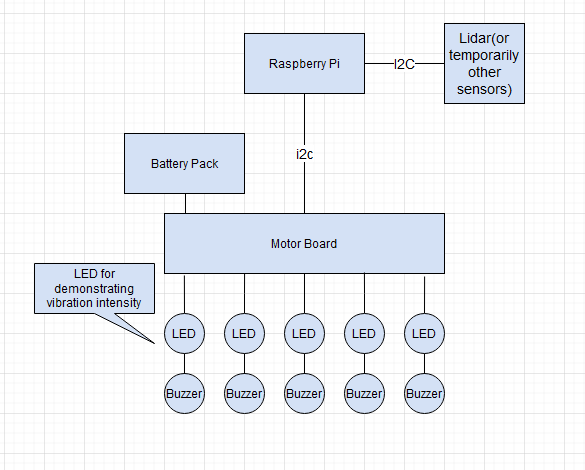
\includegraphics[width=\columnwidth]{figs/hardware-schematic.png}}
\caption{Raspberry Pi Connection Diagram}
\label{fig:hardware-schematic}
\end{center}
\vskip -5mm
\end{figure} 

\subsection{Raspberry Pi}

For this demo, we were able to successfully translate the turtlebot's LIDAR data to LED intensity, showcasing that we have the means for translating LIDAR data to vibration intensity. Using the turtlebot's Raspberry Pi, we connected the turtlebot's LIDAR to five LEDs representing mini disc vibration motors. Each LED represented one vibration motor and so from the LIDAR's data, the brighter the LED, the more the haptic feedback would theoretically vibrate.

\subsection{ROS}

To connect the hardware components of our device, we used ROS. The Turtlebot's LIDAR publishes distance data to a topic that our haptic feedback node subscribes to. Upon receiving LIDAR data, the haptic feedback node parses and translates the message to intensities and uses them to control the haptic feedback which for this demo, controls the LED intensities.

\subsection{LIDAR Data Translation}

We have written an algorithm that translates LIDAR output to a variable number of motor vibration intensities. It accomplishes this by first restricting the LIDAR's 360 degrees of data measurements to the front 180 degrees because the back 180 degrees points towards the cane's user who will consistently be close to the LIDAR. The algorithm then segments the 180 degrees of data into n-partitions and takes the minimum distance measurement of each partition to calculate the intensity at which a motor corresponding to the partition would vibrate at.

\subsection{Simulation}

We have also set up multiple simulations with humans holding lidar-attached canes to demonstrate the behavior of our product in real-world scenarios. The simulations showcase the vibration intensities through console output; reacting to the LIDAR data when objects get closer and further away from the user. The users of the Opticane also react to very close objects in the simulation by stopping their movement to demonstrate that the LIDAR data does in fact offer valuable contextual information.

The users in the simulation also swing their canes from side to side to replicate how visually impaired individuals use their white canes. The swinging programmed in the simulation follows the principles of caning techniques used by the visually impaired. \cite{rosen2014}

We also thought about the possibility of Opticane changing how white canes are swung because with the extra contextual knowledge of one's surroundings, a user might only want to know what's directly in front of them on the ground.

\subsection{3D Model}

Progress has also been made towards the design of our haptic feedback. The design team has 3D modeled Opticane's handle and in that design, we employ a grooved handle with vibration motors at each groove. We chose the grooved handle because this allows us to implement localized vibration as tactile feedback and also to know the orientation at which the cane will be held.

The grooves allow for localized vibration because they guide the fingers to specific parts of the cane so that each finger makes direct contact with a vibration motor. The grooves also make the user hold the cane in a certain orientation so we know what field of view we want to work with for our LIDAR. With this design, we use five vibration motors: one for each finger in the grooves and one for the thumb at the top of the handle. We considered just four vibration motors, one for each finger excluding the thumb, but concluded that users would probably value the LIDAR information directly in front of them much more than their sides, meaning that we would need an odd number of haptic feedback devices. We chose five motors because we are assuming that it offers enough directional granularity while also having a partition relating to the user's front. The four fingers would correlate to the left and right sides of the user while the thumb would correlate to the user's anterior. We plan on gathering feedback from users to validate the use of five motors.

The handle's dimensions are 20cm x 4.5cm x 2.3cm which loosely follow the WHO's size guidelines of handgrip length of 20cm and diameter of 2.5cm, outlined in their draft of \textit{Assistive Product Specification for Procurement}. \cite{who2020}

The grooved handle design may be uncomfortable for users who use different grips, so in the future we plan on 3D modelling handles that account for the most popular gripping methods.

\begin{figure}[tb]
\vskip 5mm
\begin{center}
\centerline{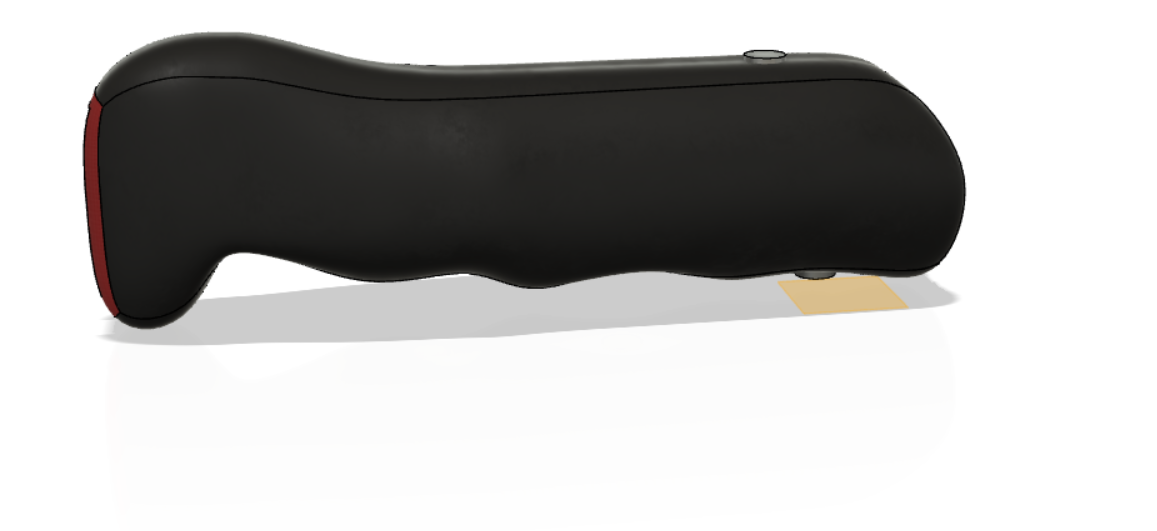
\includegraphics[width=\columnwidth]{figs/opticane-model.png}}
\caption{Opticane Handle 3D Model}
\label{fig:handle-model}
\end{center}
\vskip -5mm
\end{figure} 

\section{Evaluation}

\subsection{Quantitative}

We are using a LIDAR to detect objects that a normal white cane can't. This includes objects that are moving and those that are above the ground. The LIDAR can sense objects at a distance of 0.2 meters to 5 meters when it’s both indoors and outdoors. The LIDAR output is not affected by swinging the hand not holding the cane. The LIDAR can detect moving objects such as people walking and running and the speed at which the object moves doesn't affect the output. If the objects move from one partition to another then the LiDAR output reflects the movement. After testing, we found that swinging only affects the LIDAR’s output by shifting the partitions relative to the user but not by a significant amount. We wanted to test how color affects the LIDAR output but we couldn’t use Webots to fully simulate this. However, we found a paper that indicates we might get better performance in bright coloured objects while getting relatively worse performance with black and brown objects. \cite{bolkasMartinez2017}

We are using multiple vibrating mini disc motors for haptic feedback. To allow for localized vibration, we have decided to place the buzzers along the exterior of the handle so the user can make direct contact with each motor.

We have thought about the different places the LIDAR could be placed on the cane. The lower it is, the heavier the cane becomes, and it would also start to detect objects that the cane can already detect. The higher we place it, the LIDAR would detect fewer objects vertically because the lidar would face more horizontally as the cane is usually held slanted. Balancing these two, we have decided to put the LIDAR about 75\% above the cane’s bottom.

Since we are using a small LIDAR and small motors, we estimate that our cane would not be more than 70g heavier than the standard white cane. Most of that weight would be from the rechargeable battery and Raspberry Pi.

\subsection{Qualitative}

We have reached out to Tech Era, an organization that works with people with disabilities, and they have agreed to let us interview some of the blind people they work with. \cite{techera2020} We are waiting for ethics approval to start our interviewing process. We are planning to ask them the following questions during the interview along the lines of:
\begin{itemize}
  \item Have you ever encountered disruptions from the left or right because of things your cane cannot pick up? 
  \item What parts of your white cane do you enjoy? What are its pros and cons? 
  \item How useful would it be to have a cane to detect objects from the waist up?  
\end{itemize}

\subsection{Literature Review}

In the case study, \textit{Intelligent Mobility Cane – Lessons Learned from Evaluation of Obstacle Notification System using a Haptic Approach}, a smart cane that consists of 2 haptic vibrators on the handle was tested by visually impaired people. \cite{paritiTibdewalOh2020} “After the usability testing which took mostly around 3 minutes, the participants became comfortable with the IMC and liked the idea of communicating using haptic feedback. Some of their comments from the post-interview session are; P4: “I like the vibrators on the handle. A lot of times traffic and other noises impede my hearing. So the haptics is great.” The study found that it was easy for users to get familiarized with haptic feedback and that haptic feedback works better than audio feedback.

One area of interest we had was about the disadvantages of the white cane; where could Opticane succeed where a traditional cane could not? 
Effectiveness of the haptic feedback in telling the user there are objects/people close by. The cane itself already uses haptic feedback as Hersh, Johnson and Keating point out in their book \textit{Assistive Technology for Visually Impaired and Blind People}: “The Haptic stimulus properties made available via the cane are vibrations in the cane and force feedback.” This tells us haptic feedback is already useful as a response mechanism in the cane and we are simply extending the range of response of such feedback further than the 1m of a usual cane through the use of the LIDAR. Also, our segmentation of the visual data in 5 parts, fits well with keeping a haptic response simple which Hersh, Johnson and Keating is essential for “direct translation from visual forms to tactile forms\dots” \cite{hershJohnsonKeating2008}

Another topic of interest was what issues does swinging a white cane bring?
There was very little in the way of academic research in this field. There was a paper on the effect of swing arc width on detecting obstacles whose results were mixed at best: “participants still missed approximately 20\% of presented obstacles. This poses a serious safety concern for the vast majority of cane users\dots” \cite{kimEmersonNaghshineh2017} Additionally some anecdotal accounts to the issues with canes, such as one blind Reddit user who says “my city has terrible sidewalks and my cane gets caught constantly\dots if you aren’t quick you’ll jab yourself in the ribs or tummy\dots” \cite{reddit2021} The Clovernook Centre for the Blind also mentions this in an article saying about white canes: “They love to get stuck…leading to possible stomach jabbing.” \cite{clovernook2020} This does seem to suggest there may be some underlying problems with the swinging of canes that haven’t been looked into in an academic setting yet. It would be good in the future, for us to conduct such a study to investigate if this is an issue.

\section{Budget}
In terms of monetary budget, our group has spent about £30 on hardware components. We've only had to order our LIDAR unit as the other parts are available in Appleton. For technician time, we've spent one hour of each week with supervised lab time working on the Raspberry Pi and turtlebots in Appleton. This accounts for about three hours of technician time. In addition to that, we've attended office hours for Christopher McGreavy, Julian Habekost, Ryan Bowler, and Benedetta Catanzariti. In total, by tallying all of the story points in our Trello Board for this demo, we've spent about 248 hours working.

\section{Video}
\url{https://uoe-my.sharepoint.com/:v:/g/personal/s1870157_ed_ac_uk/EZQxP0igLnBNufvmZX7LWhMB7vwyGepkUEaAldOSFYKd-g?e=u2Qrde}


%% Include any references in a bibliography

\bibliography{references}

\end{document} 

